\documentclass[11pt,a4paper]{article}
\usepackage[margin=2.5cm]{geometry}
\usepackage{fontspec}
\usepackage{amsmath}
\usepackage{booktabs}
\usepackage{array}
\usepackage{enumitem}
\usepackage{multicol}
\usepackage{xcolor}
\usepackage{graphicx}
\usepackage[hidelinks]{hyperref}
\hypersetup{colorlinks=true,urlcolor=blue!60!black,linkcolor=black}
\setlist{itemsep=2pt}
\graphicspath{{../outputs/eda/figures/}}
\renewcommand{\topfraction}{0.85}
\renewcommand{\textfraction}{0.1}
\renewcommand{\floatpagefraction}{0.8}

\title{\textbf{N24News -- Multimodal News Classification}\\[4pt]\large Dataset Proposal -- Assignment 3 (Milestone M1)}
\author{Group G-10\\[2pt]\small CO3133 Deep Learning, Ho Chi Minh City University of Technology (HCMUT)}
\date{November 2026}

\begin{document}
\maketitle

\section{Dataset Name, Source, Version, and License}

\begin{description}[leftmargin=0pt,itemsep=1pt]
\item[Dataset name:] N24News: A New Dataset for Multimodal News Classification.
\item[Source:] \url{https://github.com/billywzh717/N24News}; paper: \href{https://arxiv.org/abs/2108.13327}{arXiv:2108.13327}.
\item[Authors:] Zhen Wang, Xu Shan, Xiangxie Zhang, and Jie Yang (LREC 2022).
\item[Version:] Official archive \texttt{N24News.zip} linked from the repository README (Google Drive), accessed on 17 November 2026. The primary metadata file is \texttt{news/nytimes.json} (61,235 articles), accompanied by the official split files \texttt{nytimes\_train/dev/test.json} and an \texttt{images/} folder.
\item[License:] The repository contains no license file. The data consist of New York Times content redistributed by the authors for academic research; they will be used only for this course project and will not be redistributed.
\end{description}

The dataset contains news articles published by The New York Times between 2010 and 2020. Each article provides a headline, an abstract, a body, a main image, and an image caption, and is assigned one of 24 news sections, making the dataset suitable for supervised, multiclass image--text classification.

\section{Task Definition}

The objective is to classify a news article, represented by its main image and its text, into one of 24 news categories:

\begin{multicols}{3}
\begin{itemize}[leftmargin=1.5em]
\item Health
\item Science
\item Television
\item Travel
\item Movies
\item Dance
\item Real Estate
\item Economy
\item Sports
\item Theater
\item Opinion
\item Music
\item Books
\item Technology
\item Style
\item Food
\item Art \& Design
\item Global Business
\item Media
\item Fashion \& Style
\item Well
\item Education
\item Your Money
\item Automobiles
\end{itemize}
\end{multicols}

These are exactly the 24 values of the \texttt{section} field in the released data. The task is formulated as a single-label, 24-class image--text classification problem.

\begin{description}[leftmargin=0pt,itemsep=1pt]
\item[Modalities:] (A) text and (B) image. Both come from the same news article, so every pair is linked by the same entity.
\item[Input:] The headline and abstract fields joined as a text pair (modality A), and the main article image resized to 224$\times$224 (modality B).
\item[Output:] One of the 24 news categories.
\item[Annotation type:] One section label per article, assigned by the newspaper's section structure rather than by manual annotation. The free-text caption is metadata, not a label.
\end{description}

The remaining fields are the article body and the image caption. These fields will be retained for dataset examination and ablation studies but excluded from the primary model input. In particular, the body will not be used because it is long (median 809 words) and highly informative on its own, which would reduce the measurable contribution of the image. The caption will not be used because it describes the image content in text and would leak visual information into the text modality; it will only be added in a dedicated ablation. Figure~\ref{fig:samples} shows one example pair from each of eight categories.

\begin{figure}[htbp]
\centering
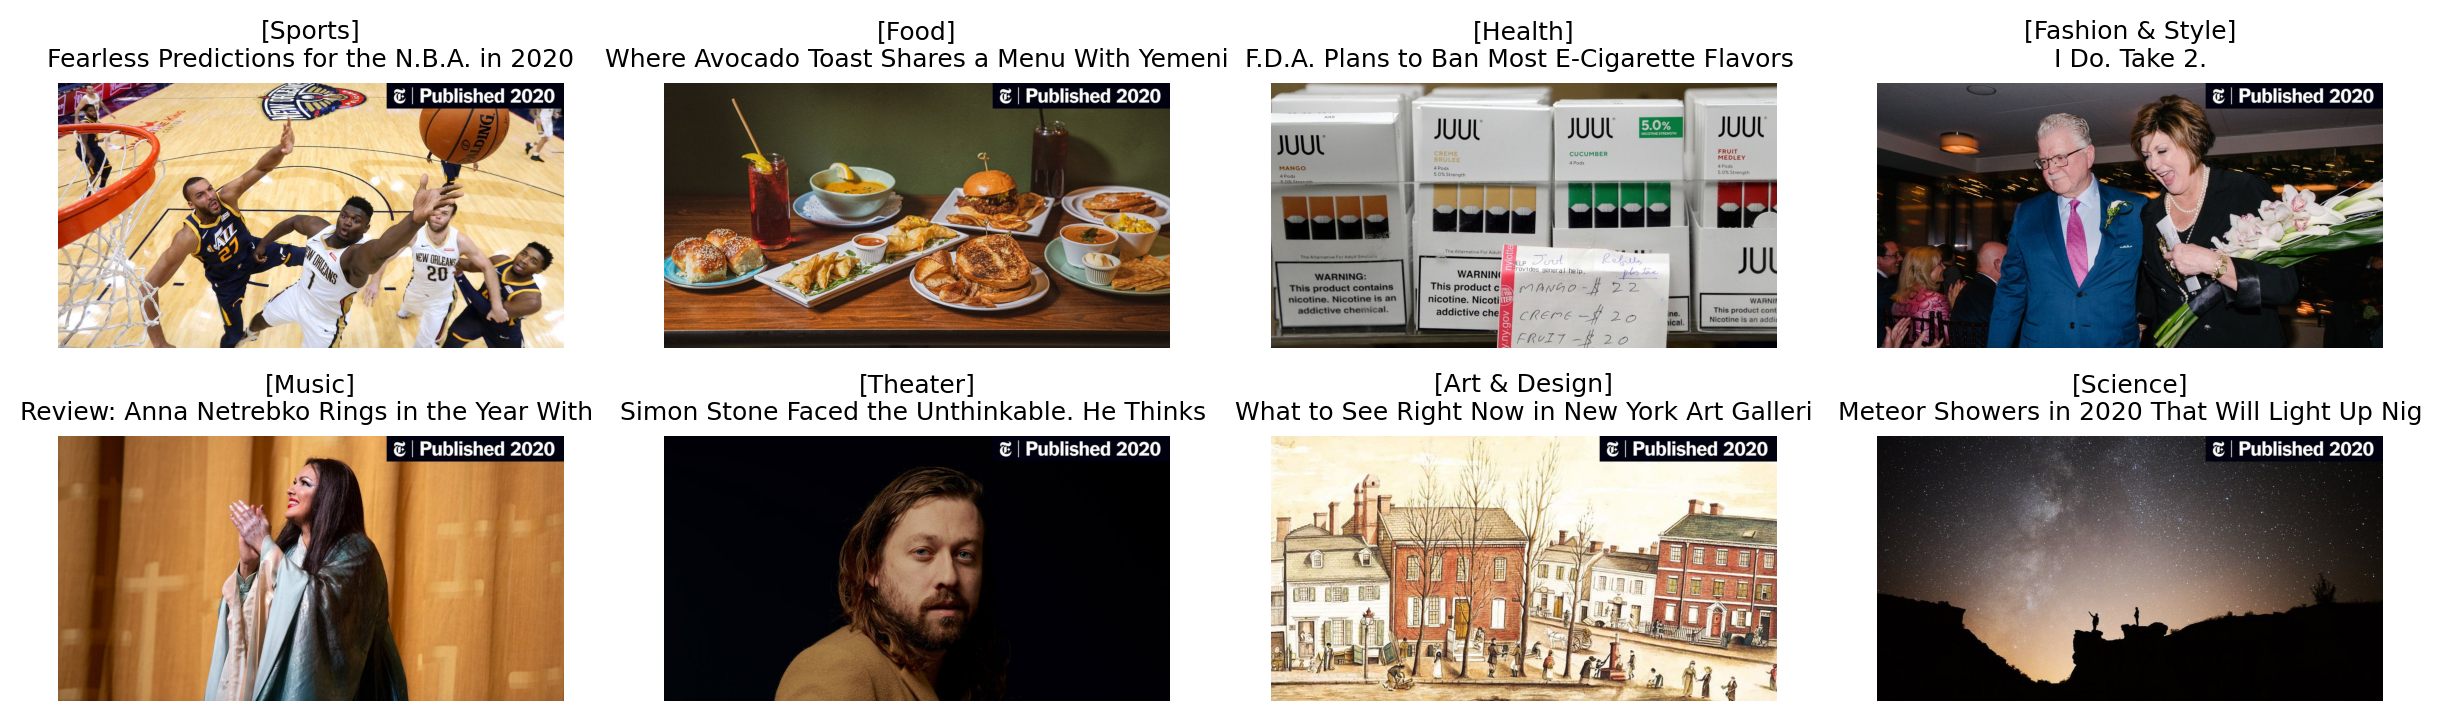
\includegraphics[width=\linewidth]{sample_pairs_compact.png}
\caption{Example image--text pairs (category and headline above each image). Note the ``Published YYYY'' badge in the top-right corner of every thumbnail.}\label{fig:samples}
\end{figure}

\section{Dataset Size and Preliminary Analysis}

The released metadata file contains 61,235 image--text pairs. The authors also provide an official split of 48,988 / 6,123 / 6,124 articles. Because this split leaks duplicates almost as much as a random split (Section~\ref{sec:dups}), we will instead use our own duplicate-aware split (Section~\ref{sec:split}), whose resulting sizes are summarized in Table~\ref{tab:overview}.

\begin{table}[htbp]
\centering
\caption{Dataset overview per split (duplicate-aware split, seed 42).}\label{tab:overview}
\begin{tabular}{lccc}
\toprule
\textbf{Property} & \textbf{Training set} & \textbf{Validation set} & \textbf{Test set}\\
\midrule
Number of samples & 49,340 & 5,980 & 5,915\\
Share of valid pairs & 80.57\% & 9.77\% & 9.66\%\\
Number of target classes & 24 & 24 & 24\\
Articles in duplicate groups & 3,060 & 284 & 330\\
Publication period & 01/2010--12/2020 & 01/2010--12/2020 & 01/2010--12/2020\\
\bottomrule
\end{tabular}
\end{table}

All three splits cover the full publication period, but the articles are far from uniformly distributed in time (Figure~\ref{fig:period}): fewer than about 250 articles per month were collected before 2016, compared with roughly 1,000--1,500 per month in 2018--2020, so the large majority of the data comes from the last five years. Because our split is not temporal, this concentration does not create a train--test shift, but it means that conclusions mainly reflect recent news content.

\begin{figure}[htbp]
\centering
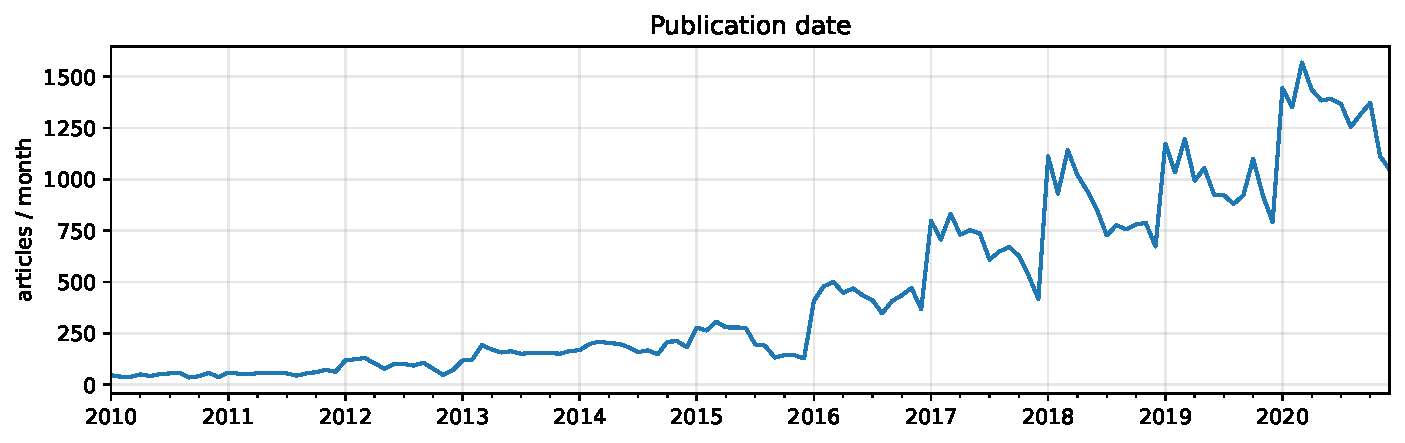
\includegraphics[width=\linewidth]{publication_period.pdf}
\caption{Articles per month, based on the date in the article URL (60,803 of 61,235 articles have a parsable date).}\label{fig:period}
\end{figure}

Table~\ref{tab:validity} reports pair counts and missing-modality rates. No image is missing or unreadable, and no article has an empty headline or abstract, so all \textbf{61,235 pairs are valid} and no sample needs to be removed. Captions are missing for 303 articles (0.49\%) and bodies for 15 articles, which does not affect the primary experiment because neither field is used as model input.

\begin{table}[htbp]
\centering
\caption{Pair counts and missing-modality rates.}\label{tab:validity}
\begin{tabular}{lcc}
\toprule
\textbf{Check} & \textbf{Articles} & \textbf{Rate}\\
\midrule
Image--text pairs in \texttt{nytimes.json} & 61,235 & 100\%\\
Missing image file & 0 & 0\%\\
Corrupt or unreadable image & 0 & 0\%\\
Empty headline / empty abstract & 0 / 0 & 0\%\\
Empty caption (ablation field only) & 303 & 0.49\%\\
Empty body (ablation field only) & 15 & 0.02\%\\
Missing label & 0 & 0\%\\
\midrule
\textbf{Valid pairs kept} & \textbf{61,235} & \textbf{100\%}\\
\bottomrule
\end{tabular}
\end{table}

\subsection{Class Distribution}

Contrary to the impression that N24News is fully balanced, the released data are capped at 3,001 articles per class: 17 classes reach the cap, while seven classes are smaller, down to 681 articles for Well (Table~\ref{tab:classes}). The ratio between the largest and smallest class is 4.41.

\begin{table}[htbp]
\centering
\caption{Class distribution of all valid pairs and of the training split.}\label{tab:classes}
\begin{tabular}{lcc}
\toprule
\textbf{Category} & \textbf{All pairs} & \textbf{Training set}\\
\midrule
17 classes at the cap$^{*}$ & 3,001 each (4.90\%) & 2,313--2,483\\
Style & 2,681 (4.38\%) & 2,165\\
Automobiles & 1,825 (2.98\%) & 1,468\\
Economy & 1,761 (2.88\%) & 1,438\\
Your Money & 1,263 (2.06\%) & 1,014\\
Global Business & 1,182 (1.93\%) & 944\\
Education & 825 (1.35\%) & 684\\
Well & 681 (1.11\%) & 557 (1.13\%)\\
\midrule
\textbf{Total} & \textbf{61,235} & \textbf{49,340}\\
\bottomrule
\end{tabular}

\smallskip
{\footnotesize $^{*}$Health, Science, Television, Travel, Movies, Dance, Real Estate, Sports, Technology, Theater, Opinion, Music, Books, Art \& Design, Media, Food, Fashion \& Style.}
\end{table}

The smallest classes are also semantically close to large ones: Well overlaps with Health, Style with Fashion \& Style, and Economy, Your Money, and Global Business share financial content. Therefore, the experiment will report both accuracy and macro-averaged F1-score. Macro-F1 is particularly important because it gives each news category equal weight regardless of its sample count. Figure~\ref{fig:classes} shows the per-class counts in the training and test splits; the test set contains between 52 (Well) and 379 (Art \& Design) articles per class.

\begin{figure}[htbp]
\centering
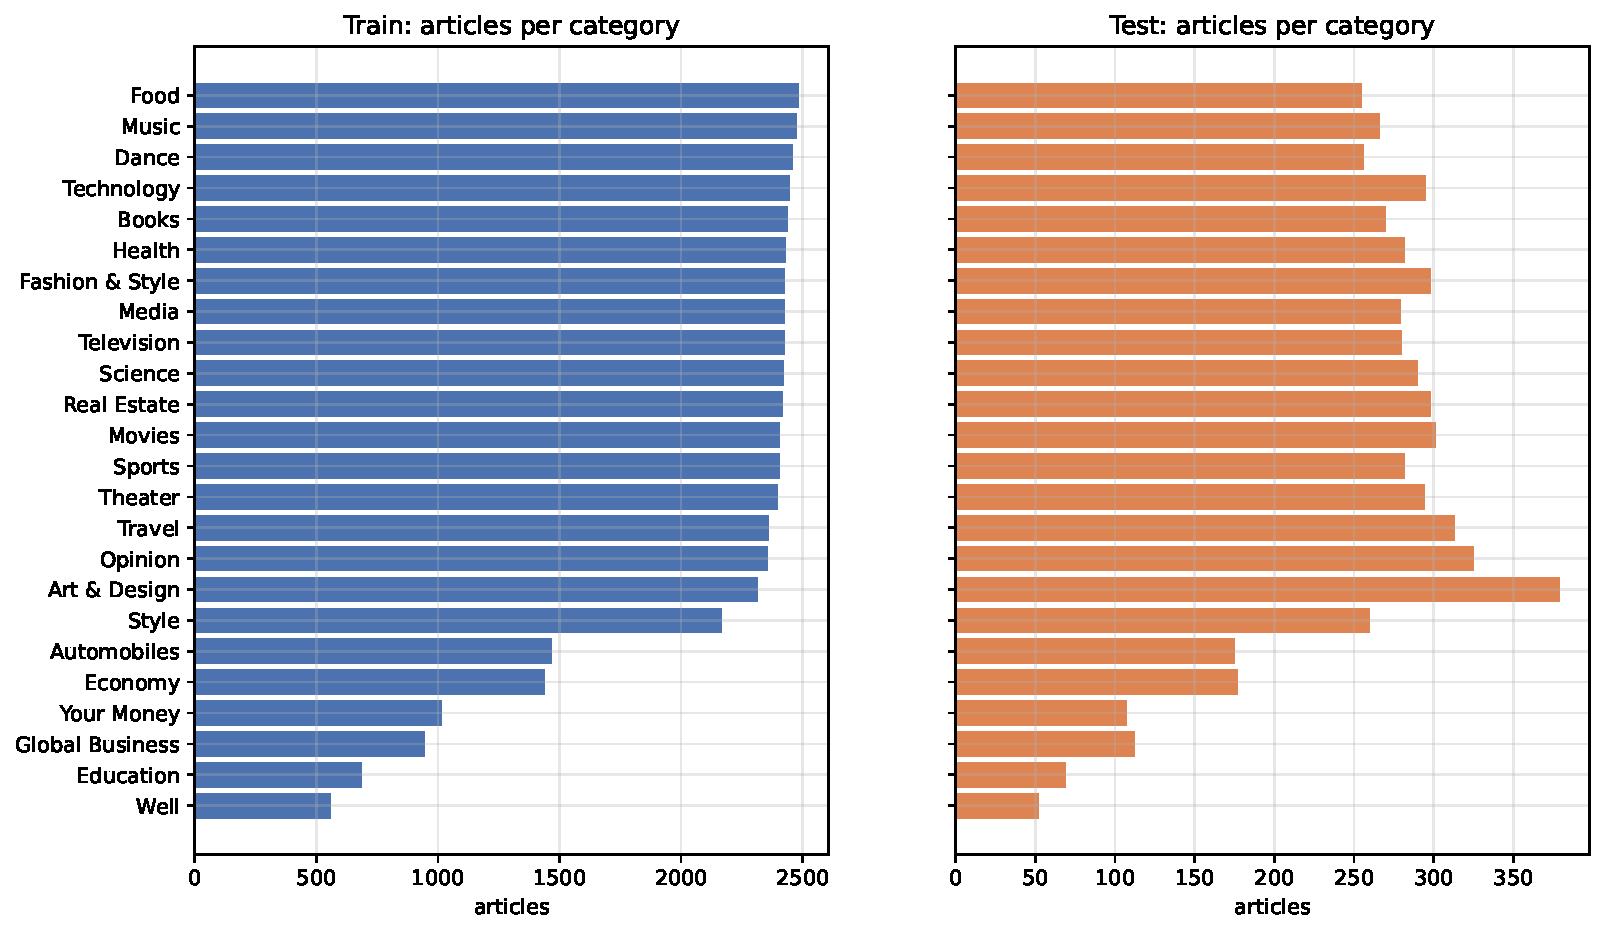
\includegraphics[width=0.9\linewidth]{class_distribution.pdf}
\caption{Articles per category in the training and test splits.}\label{fig:classes}
\end{figure}

\subsection{Text Characteristics}

Table~\ref{tab:text} summarizes text lengths in whitespace-separated words and in RoBERTa subword tokens.

\begin{table}[htbp]
\centering
\caption{Text-length statistics (words unless stated otherwise).}\label{tab:text}
\begin{tabular}{lccccc}
\toprule
\textbf{Field} & \textbf{Mean} & \textbf{Median} & \textbf{95th pct.} & \textbf{Max} & \textbf{Mean tokens}\\
\midrule
Headline & 8.79 & 9 & 13 & 22 & 12.86\\
Abstract & 21.28 & 22 & 30 & 61 & 27.36\\
Headline + abstract & 30.08 & 30 & 40 & 67 & 44.22\\
Caption (ablation) & 18.68 & 18 & 35 & 155 & --\\
Body (ablation) & 787.95 & 809 & 1,628 & 7,454 & --\\
\bottomrule
\end{tabular}
\end{table}

The encoded headline--abstract pair (including special tokens) has a 95th percentile of 58 tokens, a 99th percentile of 65, and a maximum of 87. Headlines are short and often written to attract attention rather than to describe the topic, while abstracts provide one or two summary sentences. Combining the two fields gives a moderately informative text signal of about 30 words that leaves room for the image to contribute, whereas the body is roughly 26 times longer. Figure~\ref{fig:length} shows the length distributions.

\begin{figure}[htbp]
\centering
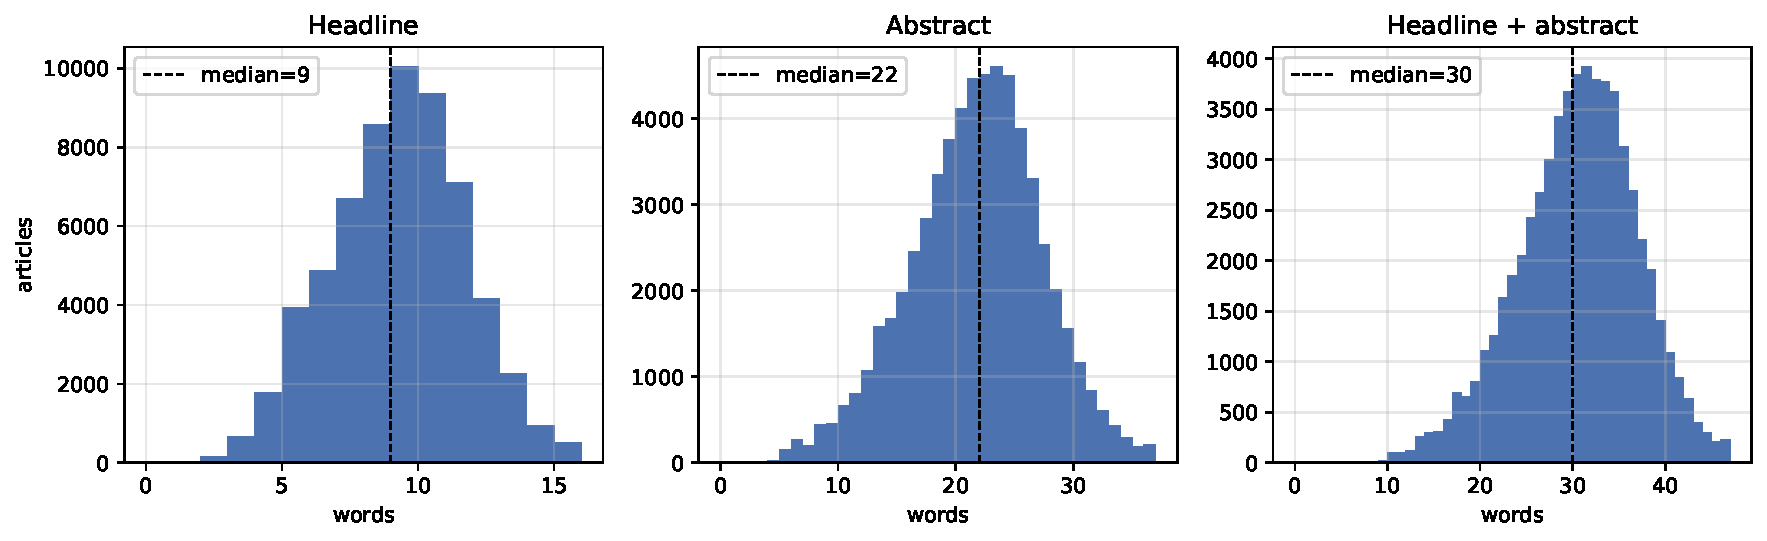
\includegraphics[width=\linewidth]{text_length.pdf}
\caption{Distribution of words per headline, abstract, and headline + abstract.}\label{fig:length}
\end{figure}

\subsection{Text and Image Preprocessing Strategy}

Preprocessing will be applied consistently to the training, validation, and test sets. For the text modality, the headline and abstract will be encoded as a RoBERTa sentence pair, with only minimal normalization (HTML entities, redundant whitespace) so that topic-bearing words are preserved. Sequences will be padded or truncated to a maximum length of \textbf{128 tokens}, which covers 100\% of the samples; padding tokens will be excluded from computation using attention masks.

For the image modality, most images are NYTimes social-sharing thumbnails with a fixed size of 1050$\times$550 pixels (median aspect ratio 1.91; 5th--95th percentile 1.57--1.91). Figure~\ref{fig:resolution} shows that a smaller second group of images is 600 pixels wide with heights of about 300--400 pixels (aspect ratio near 1.5). A total of 145 images are not RGB (85 grayscale, 42 RGBA, 17 palette, 1 LA) and will be converted to RGB, and 159 images (0.26\%) have a shorter side below 224 pixels and will be upsampled. Visual inspection shows that many thumbnails carry a small ``NYT $|$ Published YYYY'' badge in the top-right corner. Because this badge encodes the publication year rather than the topic, it could act as a shortcut feature. Resizing the shorter side to 224 pixels followed by a 224$\times$224 center crop removes the right edge of these wide images, including the badge. Images will then be normalized with the statistics of the selected pretrained image encoder. Light augmentation (random resized crop restricted to the central region and horizontal flip) will be applied to the training set only.

\begin{figure}[htbp]
\centering
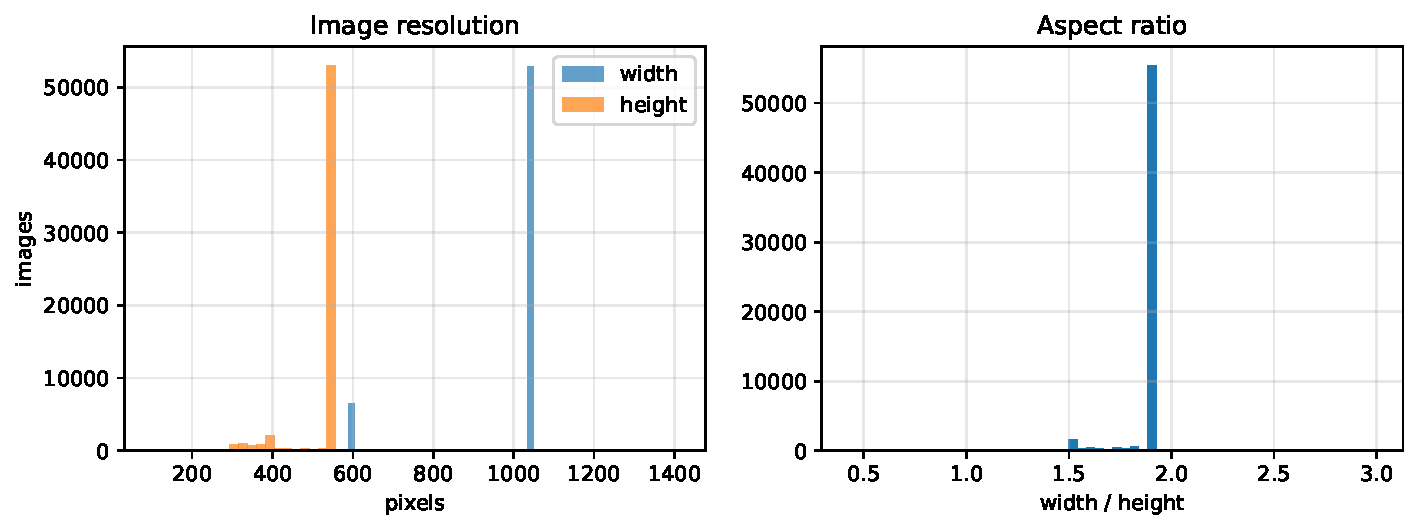
\includegraphics[width=0.95\linewidth]{image_resolution.pdf}
\caption{Image width and height (left) and aspect ratio (right) of the 61,235 images.}\label{fig:resolution}
\end{figure}

\subsection{Pair Validity, Duplicate, and Leakage Examination}\label{sec:dups}

A valid pair is defined as an image and a text that belong to the same news article; alignment is performed by the article record, which stores the image identifier, so no cross-dataset pairing is involved. Beyond missing and corrupt files (Table~\ref{tab:validity}), the examination searched for identical or near-identical images shared by different articles using a 64-bit perceptual hash (Hamming distance $\le 4$) and for repeated headlines after normalization (lower-casing, punctuation removal). Both relations were treated as edges of a graph over articles, and each connected component forms one duplicate group (Table~\ref{tab:pairs}).

\begin{table}[htbp]
\centering
\caption{Duplicate and leakage checks on the 61,235 valid pairs.}\label{tab:pairs}
\begin{tabular}{lc}
\toprule
\textbf{Check} & \textbf{Result}\\
\midrule
Articles sharing an identical perceptual hash & 1,383\\
Near-identical image pairs (distance $\le 4$) & 3,617 pairs, 2,002 articles\\
Articles with a repeated normalized headline & 1,828\\
Duplicate groups after merging & 935 groups, 3,674 articles (6.0\%)\\
Largest duplicate group & 406 articles\\
Groups with conflicting labels & 144 groups, 615 articles\\
\midrule
\multicolumn{2}{l}{\emph{Articles whose duplicate group also appears in the training set:}}\\
Random stratified split, test & 366 of 6,124 (5.98\%)\\
Official split, dev & 357 of 6,123 (5.83\%)\\
Official split, test & 335 of 6,124 (5.47\%)\\
Our duplicate-aware split, val / test & 0 / 0 (0\%)\\
\bottomrule
\end{tabular}
\end{table}

Repeated headlines mostly come from recurring columns, for example ``Recent Commercial Real Estate Transactions'' (182 articles), ``What to Cook This Week'' (145), ``What to Cook This Weekend'' (137), and ``How Much Watching Time Do You Have This Weekend?'' (100). Such templates make the text trivially predictive of the section, and reused photos make the image predictive in the same way. Figure~\ref{fig:dups} shows members of the four largest duplicate groups: they share a template headline while their images differ, which is why headline matching is needed in addition to image hashing.

\begin{figure}[htbp]
\centering
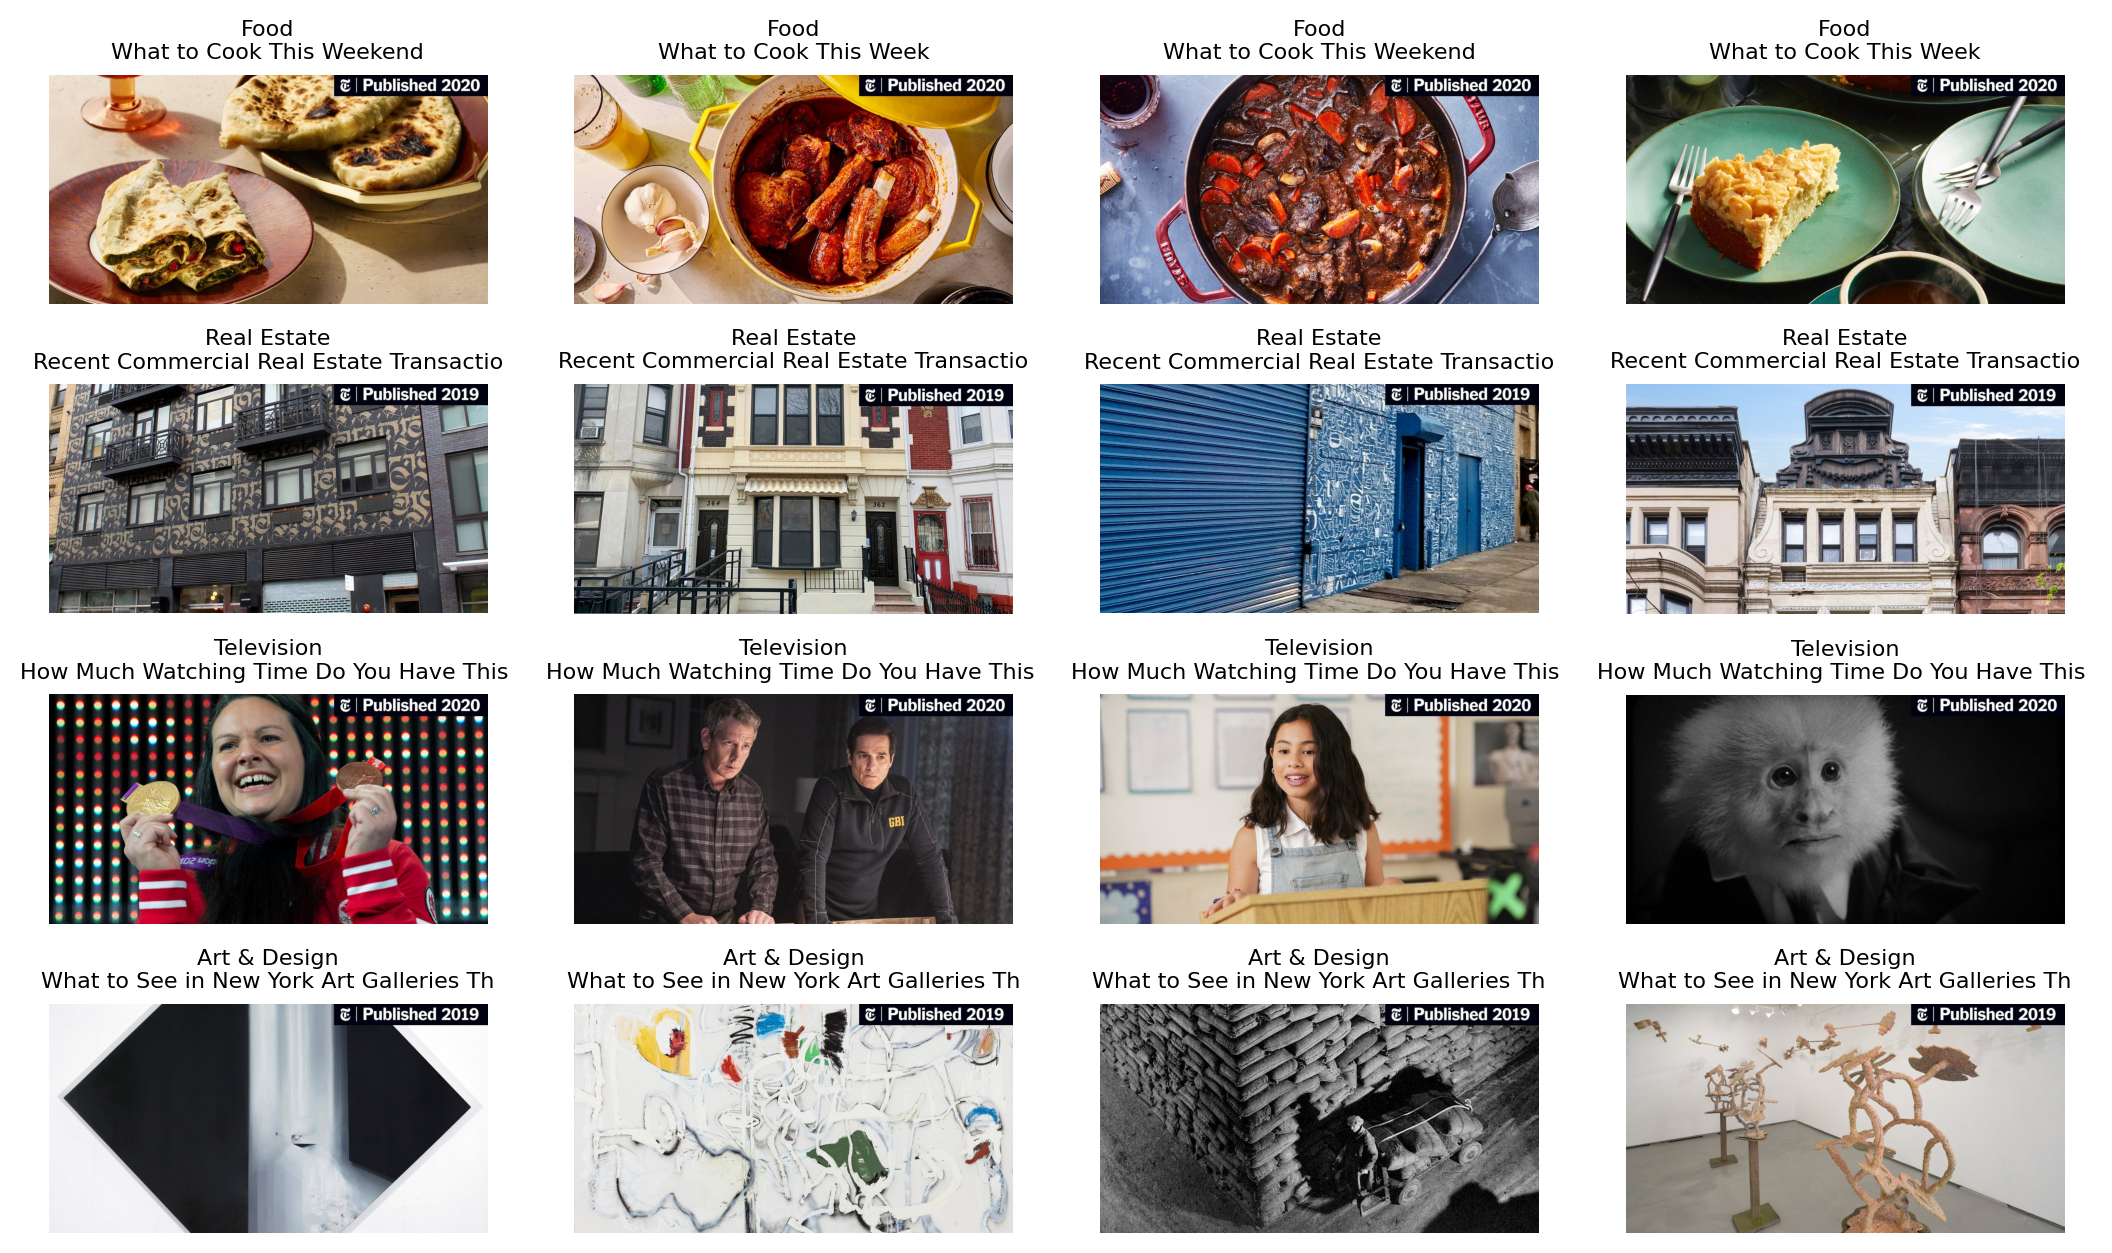
\includegraphics[width=0.9\linewidth]{duplicate_examples_compact.png}
\caption{Four articles from each of the four largest duplicate groups (one group per row).}\label{fig:dups}
\end{figure} Under a random split, 5.98\% of test articles would have a duplicate in the training set, and the official split is barely better, with 5.47\% of its test articles and 5.83\% of its dev articles affected. The test score could therefore be inflated by memorization rather than generalization. Duplicate groups will therefore be kept within a single split, and their effect will be quantified in an ablation (Section~\ref{sec:ablation}). The 144 label-conflicting groups indicate images or headlines reused across sections; they are kept, since they are genuine data, and will be examined as natural cases of conflicting evidence.

\subsection{Reference Results from the Original Paper}

The original paper reports the F1-scores in Table~\ref{tab:paper}, which motivate the choice of text fields and will serve as reference points.

\begin{table}[htbp]
\centering
\caption{F1-scores reported by Wang et al.\ (2022) on N24News.}\label{tab:paper}
\begin{tabular}{lccc}
\toprule
\textbf{Text field} & \textbf{Text only (F1)} & \textbf{Text + image (F1)} & \textbf{Gain}\\
\midrule
Image only & -- & 52.80 & --\\
Headline & 70.31 & 78.42 & +8.11\\
Abstract & 78.19 & 82.52 & +4.33\\
Body & 87.65 & 90.44 & +2.79\\
\bottomrule
\end{tabular}
\end{table}

The gain from adding the image decreases as the text becomes more informative. This is an important dataset characteristic because a very strong text field would hide the contribution of the visual modality. The headline + abstract configuration was therefore selected for the primary experiment as a setting where both modalities are expected to matter. Because the paper uses the official split, in which 5.47\% of test articles have a duplicate in training, these numbers will be used for orientation only and not as directly comparable results. To connect with the paper, the final models will additionally be evaluated on the official split (Section~\ref{sec:ablation}).

\section{Data Preparation and Split Strategy}\label{sec:split}

\begin{itemize}
\item \textbf{Split unit:} The duplicate group. Articles that share a near-identical image or a normalized headline form one group, and every group is assigned to exactly one split; an article without duplicates is its own group.
\item \textbf{Method:} \texttt{StratifiedGroupKFold} with 10 folds, shuffling, and seed 42; fold 0 is the test set, fold 1 the validation set, and the remaining folds the training set. The resulting article IDs are saved in \texttt{splits.csv} and reused by all models.
\item \textbf{Training data:} 49,340 pairs (80.57\%), used for model fitting.
\item \textbf{Validation data:} 5,980 pairs (9.77\%), used for hyperparameter selection, checkpoint selection, and early stopping.
\item \textbf{Test data:} 5,915 pairs (9.66\%), reserved for final evaluation.
\end{itemize}

All 24 classes appear in every split, and it was verified that no duplicate group crosses splits. The official split was not adopted because 5.47\% of its test articles and 5.83\% of its dev articles have a duplicate in its training set (Table~\ref{tab:pairs}). Because whole groups are assigned at once, per-class proportions deviate slightly from 80/10/10 (for example, the largest group of 406 articles falls into a single split). Preprocessing will include tokenization appropriate to the text encoder, consistent truncation and padding, and consistent image resizing and normalization applied identically to every split.

\textbf{Subset rules:} No subsetting will be applied: all 61,235 valid pairs are used, with no class capping, resampling, or removal of duplicates. A fixed 10\% stratified sample of the training split will be used only for debugging the pipeline, never for reported results.

\section{Planned Models}

\subsection{Text-Only Model: RoBERTa-base}

The first unimodal baseline (modality A) will be RoBERTa-base fine-tuned on the headline--abstract pair. The representation of the first token (CLS) will be passed to a 24-class classification head. This model measures how much category information is available from text alone.

\subsection{Image-Only Model: ViT-B/16 or CLIP Image Encoder}

The second unimodal baseline (modality B) will be a pretrained ViT-B/16 or the CLIP ViT-B/16 image encoder, followed by a 24-class classification head. The final choice will be made on the validation set. This model measures how much category information is available from the image alone.

\subsection{Baseline Model: Simple Concatenation Fusion}

The multimodal baseline will reproduce the fusion approach of the original paper. The CLS embedding of the text encoder and the pooled embedding of the image encoder will be concatenated and passed to a multilayer perceptron (MLP) that predicts one of the 24 categories. This late-fusion model provides a reference point for assessing the benefit of a more expressive fusion mechanism.

\subsection{Improved Model: Cross-Attention with Gated Fusion}

The improved model performs intermediate fusion: text tokens attend to image patch tokens (and vice versa) through cross-attention layers, and the resulting representations are combined with a learned gate that weighs the contribution of each modality per sample. Two training techniques will be added: auxiliary unimodal classification heads on the text and image branches, so that each encoder remains discriminative on its own, and modality dropout, in which one modality is randomly masked during training so that the model remains robust when a modality is missing or uninformative. The overall loss is
\[
\mathcal{L} = \mathcal{L}_{\text{CE}}(\hat{y}_{\text{fused}}, y) + \lambda_{T}\,\mathcal{L}_{\text{CE}}(\hat{y}_{\text{text}}, y) + \lambda_{I}\,\mathcal{L}_{\text{CE}}(\hat{y}_{\text{image}}, y),
\]
where $\lambda_T$ and $\lambda_I$ are selected on the validation set; the unimodal baselines and the concatenation baseline use only the cross-entropy term of their single head. Plain cross-entropy is the default; class-weighted cross-entropy will be considered only if minority-class F1 lags clearly on the validation set.

\textbf{Pretraining and fine-tuning strategy:} All encoders start from public pretrained checkpoints. Features of the frozen encoders are first cached to train the fusion heads cheaply; the best configurations are then fine-tuned with only the upper encoder layers unfrozen. The experiment will record the selected checkpoints, tokenizer, maximum sequence length, image resolution, learning rates, batch size, number of epochs, loss weights, modality-dropout rate, and the checkpoint-selection criterion.

\section{Controlled Experiment}

\textbf{Research question:} Does an attention-based, gated fusion model trained with auxiliary unimodal losses and modality dropout improve news category classification compared with simple concatenation fusion, and does the image provide information beyond the headline and abstract?

\textbf{Hypothesis:} Both multimodal models will achieve a higher macro-F1-score than the best unimodal model, and the improved fusion model will achieve a higher macro-F1-score than the concatenation baseline because cross-attention and gating allow the model to exploit image--text interactions and to down-weight an uninformative modality.

\textbf{Independent variable:} The modality configuration and fusion strategy: text only, image only, concatenation fusion, and cross-attention with gated fusion.

\textbf{Controlled factors:} All models will use the same training, validation, and test article IDs, the same target labels, the same text fields, the same image preprocessing, and the same evaluation metrics. Validation-based model selection will follow a predefined criterion for each model. Each configuration will be trained with 3 random seeds, and the mean and standard deviation will be reported.

\textbf{Primary decision criterion:} Compare test macro-F1-score after selecting checkpoints and hyperparameters using only the training and validation data; a difference is considered meaningful only if it exceeds the standard deviation across seeds. Accuracy, per-class F1-scores, and the confusion matrix will provide supporting evidence. If the multimodal models do not outperform the unimodal ones, the causes will be analyzed with data properties and experimental evidence.

The experiment will also examine errors between semantically neighboring categories, such as Fashion \& Style and Style, Health and Well, and Economy, Your Money, and Global Business. These categories may be difficult to distinguish because they cover overlapping topics and may use visually similar images.

\subsection{Ablation Studies}\label{sec:ablation}

Each ablation changes a single factor relative to the main configuration, keeps all other factors fixed, and uses the same decision criterion. The ablations will be conducted on the validation set and the final configurations reported on the test set:

\begin{itemize}
\item \textbf{Text field:} Headline only, abstract only, headline + abstract, and body.
\item \textbf{Caption:} Adding the image caption to the text input, to measure visual-content leakage through text.
\item \textbf{Fusion type:} Concatenation, gated fusion without cross-attention, and cross-attention with gated fusion.
\item \textbf{Auxiliary losses:} The improved model with and without auxiliary unimodal losses.
\item \textbf{Missing modality at test time:} Removing the image or the text at inference, with and without modality dropout during training.
\item \textbf{Split strategy:} The duplicate-aware split versus the official split (5.47\% of test articles with a duplicate in training) and a random split (5.98\%), to quantify score inflation caused by duplicates and to relate our results to the numbers reported in the paper.
\end{itemize}

\section{Evaluation Metrics and Error Analysis}

The primary metrics will be:

\begin{itemize}
\item \textbf{Macro-F1-score:} The unweighted mean of the F1-scores across all 24 categories; this is the main metric.
\item \textbf{Accuracy:} The proportion of test samples assigned the correct category.
\item \textbf{Per-class precision, recall, and F1-score:} To identify categories for which the model performs poorly, especially the small classes Well, Education, Global Business, and Your Money.
\item \textbf{Confusion matrix:} To examine systematic confusion between news categories.
\end{itemize}

All metrics will be reported as the mean and standard deviation over 3 seeds. The analysis will present qualitative examples of \emph{support} cases, in which a unimodal model fails but fusion succeeds, and \emph{conflict} cases, in which the image and the text point to different categories (including the label-conflicting duplicate groups). Error analysis will cover generic or stock images, headlines whose wording does not reflect the topic, recurring-column templates, and articles that plausibly belong to several categories. The learned gate values will be inspected to analyze when the model relies on the image versus the text.

The report will avoid treating high overall accuracy alone as evidence of robust performance. Results will be interpreted alongside per-class metrics, the missing-modality results, and the duplicate-aware versus random split comparison.

\section{Compute-Cost Analysis}

All models will be trained on Kaggle or Google Colab with an NVIDIA T4 GPU. Encoding the 61,235 pairs once with each frozen encoder makes the subsequent training of fusion heads inexpensive; partial fine-tuning is reserved for the best configurations. The total budget is estimated at approximately 20--30 GPU-hours, including three seeds for the main models and the ablations. The following will be recorded:

\begin{itemize}
\item Number of trainable parameters and total parameters for each model.
\item Feature-caching time, training time per epoch, and total training time.
\item Peak GPU memory usage.
\item Inference latency or throughput on a fixed number of test samples.
\item Batch size, maximum sequence length, image resolution, optimizer, and learning rate.
\item Number of epochs, unfrozen layers, and the checkpoint-selection procedure.
\end{itemize}

The cross-attention model is expected to be computationally heavier than concatenation fusion, while it may provide stronger classification performance. The actual trade-off will be measured rather than assumed.

\section{Expected Outcome and Limitations}

This project is expected to establish a reproducible comparison between unimodal models, a simple concatenation fusion baseline, and an improved attention-based fusion model for news category classification. The comparison will quantify how much the image contributes beyond the headline and abstract, and whether the improved fusion justifies its additional computational cost.

Several limitations will be acknowledged. First, the category labels are derived from the newspaper's section structure and overlap between related sections, as shown by the 144 label-conflicting duplicate groups. Second, many news images are generic or loosely related to the article topic, which limits the information available from the visual modality, and the thumbnail badge requires care to avoid a shortcut. Third, seven classes are noticeably smaller than the others (down to 52 test articles for Well), so their per-class scores will have higher variance. Fourth, results depend on the selected text fields and on the duplicate-aware split, so they are not directly comparable with the numbers reported in the original paper. Finally, conclusions drawn from New York Times articles published between 2010 and 2020 may not generalize to other news sources, languages, or time periods.

If N24News cannot be processed within the available resources, CrisisMMD will be used as a fallback dataset. It provides paired tweets and images for humanitarian classification with 8 categories, and it will be split by crisis event to avoid leakage between events.

\section{Summary}

The proposed task uses 61,235 image--text pairs from N24News to study 24-class news category classification with the headline + abstract as text input and the main article image as visual input. Preliminary analysis shows complete modalities with no missing or corrupt pairs, a moderate class imbalance (ratio 4.41), short text inputs (median 30 words, at most 87 tokens), standardized 1050$\times$550 thumbnails with a year badge, and 6.0\% of articles in duplicate groups, which both a random split (5.98\% of test articles) and the official split (5.47\%) leak into the test set. A duplicate-aware stratified 80/10/10 split resolves this leakage.

The project will compare text-only RoBERTa-base, an image-only ViT-B/16 or CLIP encoder, a concatenation fusion baseline, and an improved cross-attention model with gated fusion, auxiliary unimodal losses, and modality dropout. Macro-F1-score will be the principal evaluation metric, supplemented by accuracy, per-class analysis, confusion matrices, support and conflict case studies, ablation studies, error analysis, and compute-cost measurements. This design provides a clear experimental comparison while accounting for the dataset's characteristics and limitations.

\end{document}
